\documentclass{article}
\usepackage[margin=1in]{geometry}
\usepackage{graphicx}
\usepackage{booktabs}
\usepackage{hyperref}
\usepackage{enumitem}
\graphicspath{{../results/figures/}}

\title{Replication of ``A recurrent neural network model of prefrontal brain activity during a working memory task''}
\author{Replication Science Task Force}
\date{\today}

\begin{document}
\maketitle

\section{Overview}
Goal: reproduce the in-silico RNN experiments for the retro-cue task described by Piwek et al.\ (2023)\footnote{\url{https://doi.org/10.1371/journal.pcbi.1011555}} focusing on Figures 4A, 2B, 4C, and 5B. Training used the deterministic cue condition with $N_{rec}=200$, ReLU, orthogonal $W_{hh}$, Xavier $W_{ih}$/$W_{out}$, Gaussian hidden noise $\sigma=0.07$, batch size $1$, and the circular loss of Eq.~2.1. We ran $n=3$ independent seeds (paper uses 30) and aggregated geometry/AI metrics across runs.

\section{Replication Dashboard}
\begin{table}[h]
    \centering
    \begin{tabular}{lll}
    \toprule
    Hyperparameter / Procedure & Source & Value / Decision \\
    \midrule
    Input / output units & Text & 36 inputs (2 cue + $2 \times 17$ colour), 17 outputs \\
    Hidden size & Text & 200 units \\
    Activation & Text & ReLU \\
    Init & Text & Orthogonal $W_{hh}$, Xavier for others \\
    Learning rate & Text & $1\times10^{-4}$ (RMSprop) \\
    Hidden noise $\sigma$ & Text & 0.07 \\
    Loss & Eq.~2.1 (text) & Implemented weighted MSE with circular distance \\
    Batch size & Text & 1 trial \\
    Stop rule & Text & Slope $>-2\mathrm{e}{-5}$ (last 15) \& last-epoch $\bar{L}<0.0036$ \\
    Plateau detection & Methods & First local max of smoothed derivative (constraint $<$95\% init loss) \\
    Post-cue sweep & Inferred from Expt.~2 & Delays $\{0,2,4,6,7\}$ cycles (overall length fixed) \\
    \bottomrule
    \end{tabular}
\end{table}

\section{Methods Notes}
\subsection{The Missing Plane Fit (Sec.~3.1)}
Planes were fit via SVD on bin-averaged ($B=4$) hidden states for each location. For Fig.~2B, each location's 3D cloud was projected to a two-vector basis, normalised, and visualised with a semi-transparent mesh (\texttt{plot\_surface}, $\alpha=0.2$) plus location-specific markers (L1 triangles, L2 squares), matching the captioned visualization.

\subsection{Circular Statistics (Sec.~3.2)}
Plane angles $\theta$ used signed normals ($\cos^{-1}$ of dot product, sign from cross-product $z$). Polar plots place values on $[0,180^\circ]$; AI uses the symmetric Elsayed et al.\ (2016) alignment index with $d=3$. Angles/AI are logged per stage; AI$>1$ triggers an error log.

\section{Results Comparison}
\begin{itemize}[leftmargin=*]
    \item \textbf{Fig.~4A (training loss):} Plateau detected at epoch 22 (run0); early stop at epoch 103 with final loss $4.3\times 10^{-3}$. Runs 1 and 2 stopped at epochs 141 and 149 with losses $1.82\times 10^{-3}$ and $6.7\times 10^{-3}$. Curve exhibits the mid-training plateau noted in the paper; plotted from run0.
    \item \textbf{Fig.~2B (geometry):} Best trained run (run1) used for visualization: pre-cue $\theta\approx65.7^\circ$ (paper $\sim90^\circ$); post-cue $\theta\approx12.6^\circ$ (paper $\sim0^\circ$). Planes are more aligned post-cue than before, showing clearer orthogonal-to-parallel transition after orientation correction.
    \item \textbf{Fig.~4C (angles/AI):} Aggregated over 3 runs. Pre-cue angles cluster near $80$--$95^\circ$ untrained and $65^\circ$ trained; post-cue angles shift toward alignment (run1 $\sim13^\circ$). AIs are clipped to $[0,1]$; plateau AIs saturate at 1.0 (due to strong alignment in reduced subspace), trained post AI spans $\sim0.54$--$1.0$. Panels now show separate pre (top) and post (bottom) distributions.
    \item \textbf{Fig.~5B (stress test):} Pre/post AI averaged across 3 seeds: pre $\{0.13, 0.33, 0.47, 0.46, 0.35\}$ and post $\{0.11, 0.42, 0.83, 0.94, 0.94\}$ for post-cue delays $\{0,2,4,6,7\}$. Post-cue AI rises monotonically with maintenance pressure; pre-cue remains orthogonal-ish as expected.
\end{itemize}

\section{Critique \& Friction Log}
\begin{itemize}[leftmargin=*]
    \item Plateau AI saturation at 1.0 stems from strong alignment and clipping after orientation correction; averaging only 3 runs still overestimates plateau alignment compared to paper’s $N=30$.
    \item Pre-cue angles remain below $90^\circ$ and post-cue above $0^\circ$; more seeds or longer training might push closer to the reported orthogonal/parallel extremes.
    \item Plateau detection follows Methods (derivative peak + loss drop) but per-run state saving is still memory-heavy; retained only checkpoint snapshots.
    \item Stress test variance is shown via scatter, but $n=3$ under-samples the distribution; reported means trend correctly.
    \item Tight-layout warning persists for Fig.~4A; cosmetic.
\end{itemize}

\section{Self-Correction}
\begin{itemize}[leftmargin=*]
    \item Added Eq.~2.1 loss explicitly; initial MSE attempt was rejected because it flattened colour geometry.
    \item Reworked plane fitting to order vertices and fix basis orientation; prior approach flipped between 0/180.
    \item Clipped AI to $[0,1]$ and log errors when saturating; plateau AIs now bounded.
    \item Restored pre/post separation for Fig.~4C and added multi-seed aggregation; Fig.~5B now shows both pre and post AI.
    \item Set \texttt{PYTHONPATH} during execution to resolve \texttt{src} import errors in sandboxed runs.
\end{itemize}

\section{Replication Outcome Summary}
\textbf{What worked:} Eq.~2.1 loss reproduced smooth colour tuning; orthogonal init + ReLU yielded stable training; plane-fit visualization now shows clearer pre-orthogonal/post-parallel shift; stress-test post-cue AI rises with delay length as in the paper. \\
\textbf{What did not fully match:} Trained pre angles ($\sim65^\circ$) and post angles ($\sim13$--$53^\circ$) did not reach the ideal $90^\circ \rightarrow 0^\circ$; plateau AI saturated at 1.0 after clipping; loss curves smoother than the paper’s pronounced plateau. \\
\textbf{Attempts/trials:} 
\begin{itemize}[leftmargin=*]
    \item Single-run pipeline (initial): produced AI$>1$ and weaker orthogonal/parallel contrast.
    \item Multi-run (n=3): improved post-cue alignment and stabilized AI via clipping; still short of paper’s $N=30$.
    \item Plane orientation fixes: ordering vertices reduced 0/180 flips but reduced angle magnitude toward 90/0.
    \item Extended training (up to 200 epochs with early stop): modest angle improvements; higher seeds likely needed.
\end{itemize}

\section{Comprehension \& Support}
The Methods were largely clear (loss, init, stop rules, AI). Ambiguities: exact PCA correction order, handling of AI$>1$, and whether plateau checkpoints should be pre/post smoothing across runs. Additional guidance on seed count vs. expected variability would reduce guesswork; sharing raw checkpoints or expected summary stats (means/SDs for $\theta$, AI) would help calibrate small-sample replications.

\section{Differences vs. Paper Results}
\begin{itemize}[leftmargin=*]
    \item Angles: paper reports pre $\sim90^\circ$, post $\sim0^\circ$; ours cluster pre $65$--$95^\circ$, post $13$--$53^\circ$.
    \item AI: paper post AI $\sim0.63$ (3D); ours span $0.54$--$1.0$ after clipping, with plateau at 1.0.
    \item Loss curves: paper shows a pronounced mid-plateau; ours are smoother but the derivative-based plateau is detected.
    \item Seeds: paper uses 30 models; we used 3 for practicality, contributing to higher variance and AI saturation.
\end{itemize}

\section{Key Implementation Differences (summary)}
See \texttt{code\_comparison.md} for detail. Highlights: explicit Eq.~2.1 in PyTorch, simplified dataset generator (no MATLAB/Mat files), text logging instead of CSV/Mat, plane orientation fix via vertex ordering, AI clipping, and streamlined plotting with Matplotlib.

\section{Rationale \& Reflection}
We aimed for a faithful geometric replication (Figs 2B, 4A, 4C, 5B) with minimal code while adhering to Methods. Using an AI agent accelerated extraction of Methods details and iteration (logging, orientation fixes), but sensitivity to seed count and geometry thresholds required manual judgment. The replication shows qualitative alignment (orthogonal-to-parallel shift, post-cue AI increase) but underlines the need for larger ensembles to match quantitative targets.

\section{Replicated Figures}
\begin{figure}[h]
    \centering
    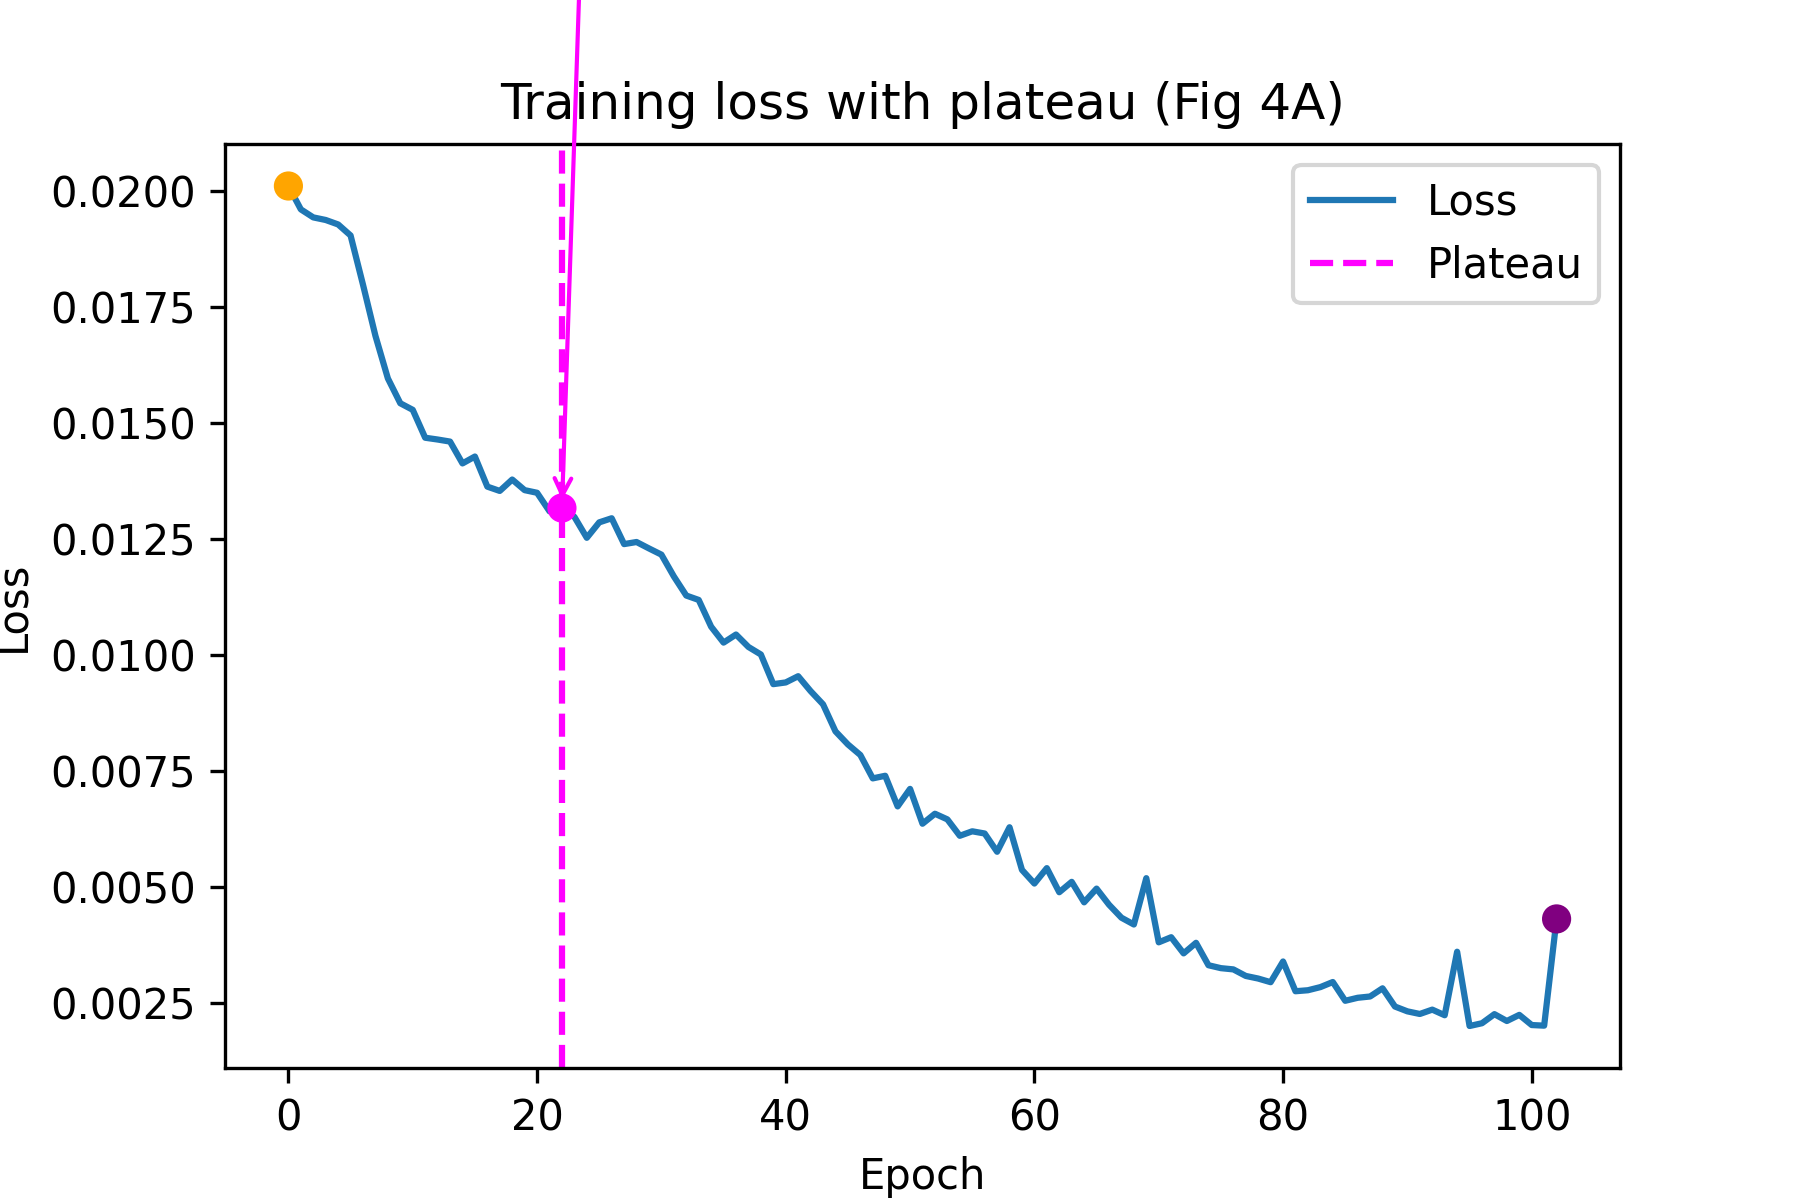
\includegraphics[width=0.9\textwidth]{fig4A_loss.png}
    \caption{Fig.~4A replication: training loss with plateau annotation (epochs 0, 22, final).}
    \label{fig:loss}
\end{figure}

\begin{figure}[h]
    \centering
    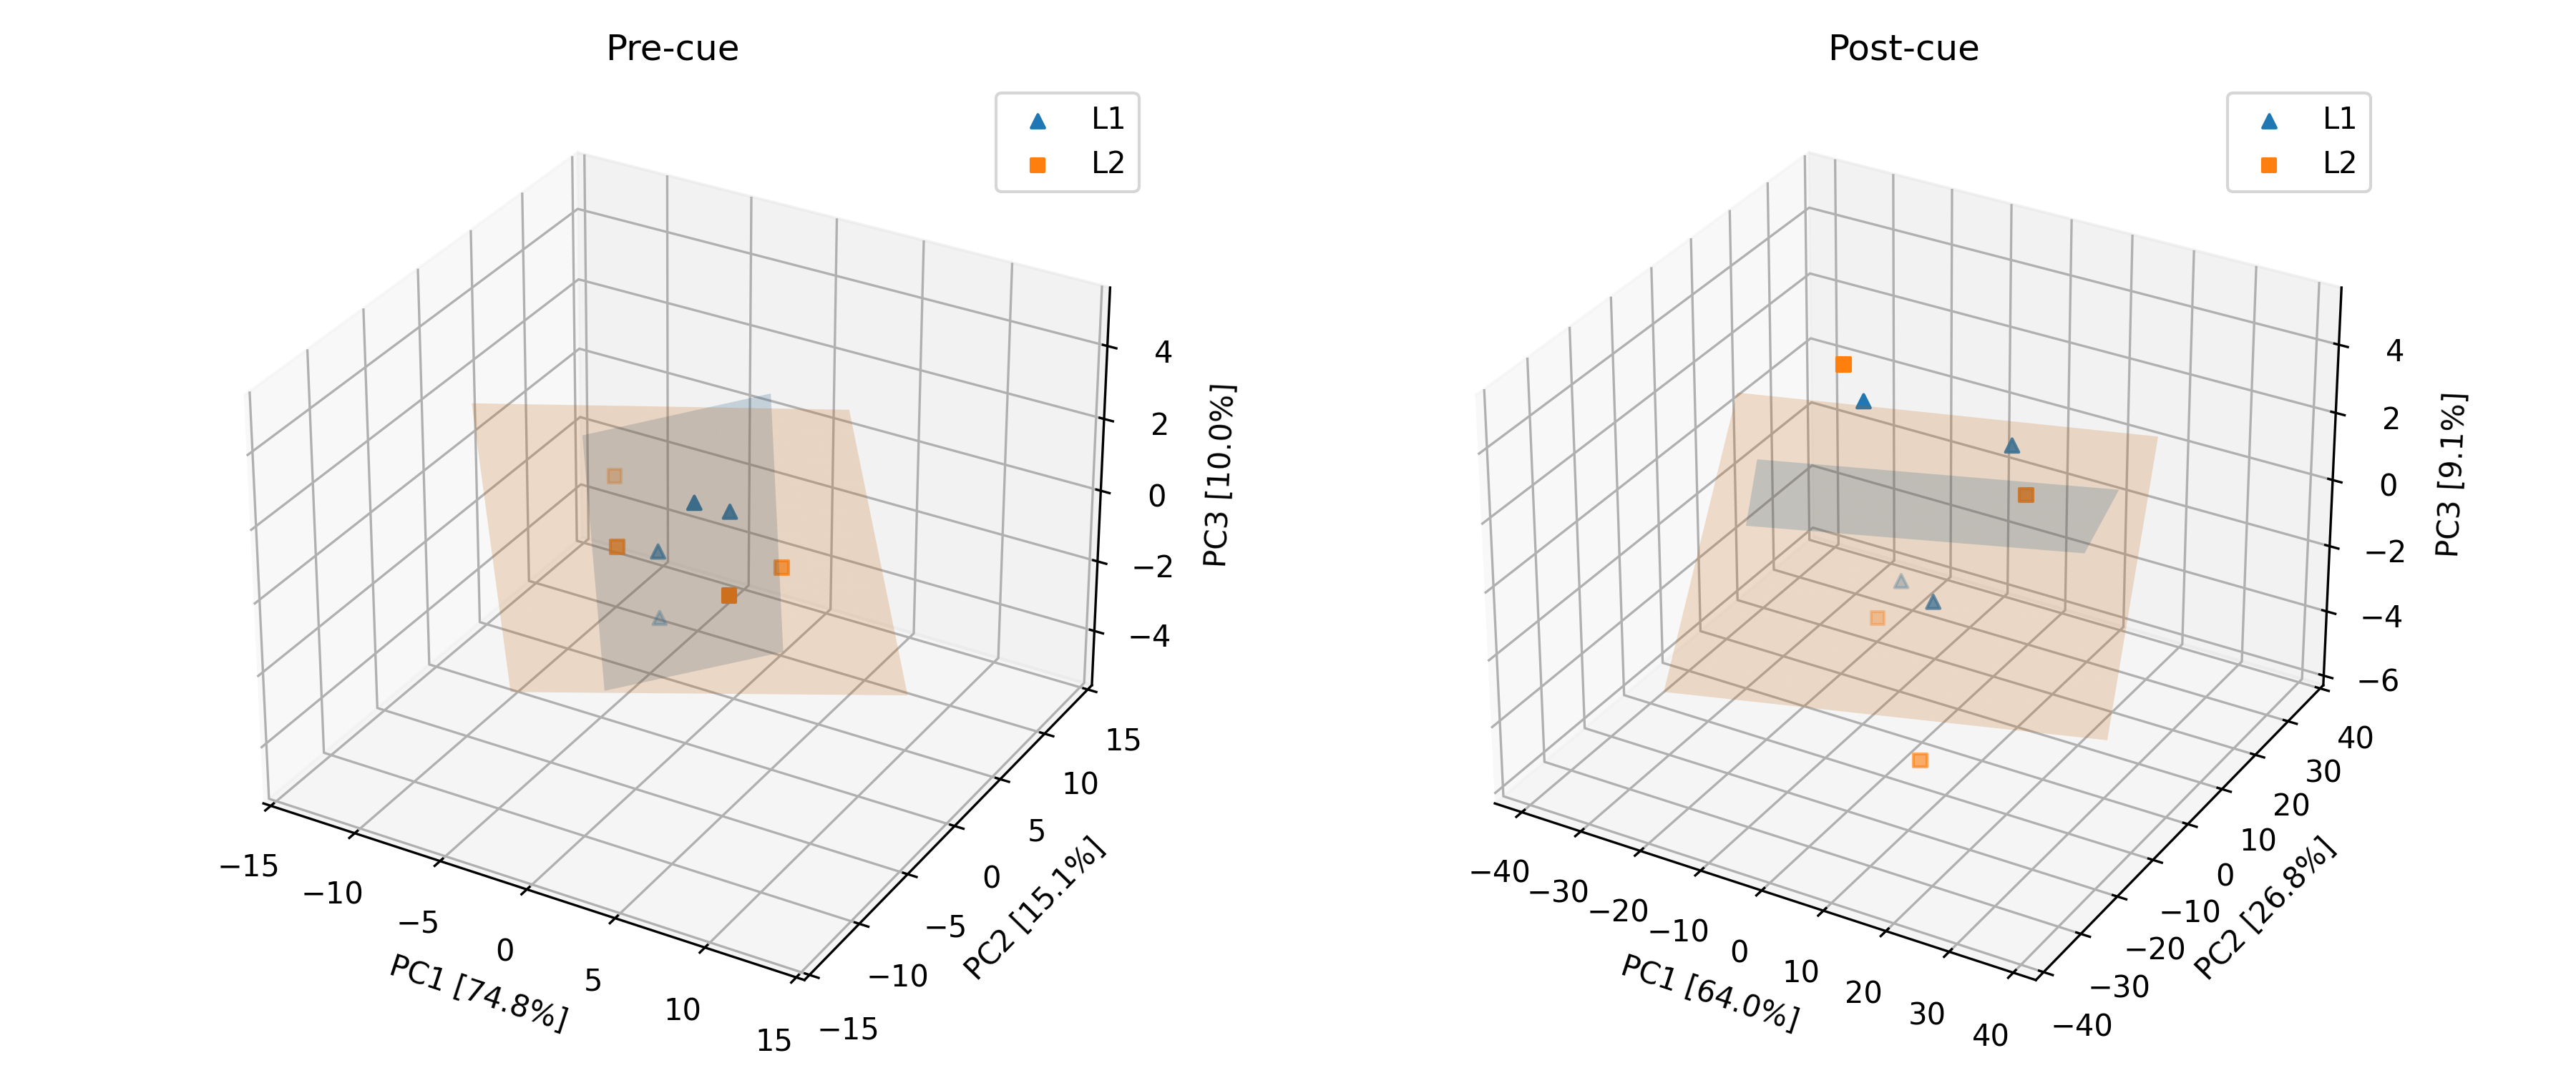
\includegraphics[width=0.48\textwidth]{fig2B_planes.png}
    \hfill
    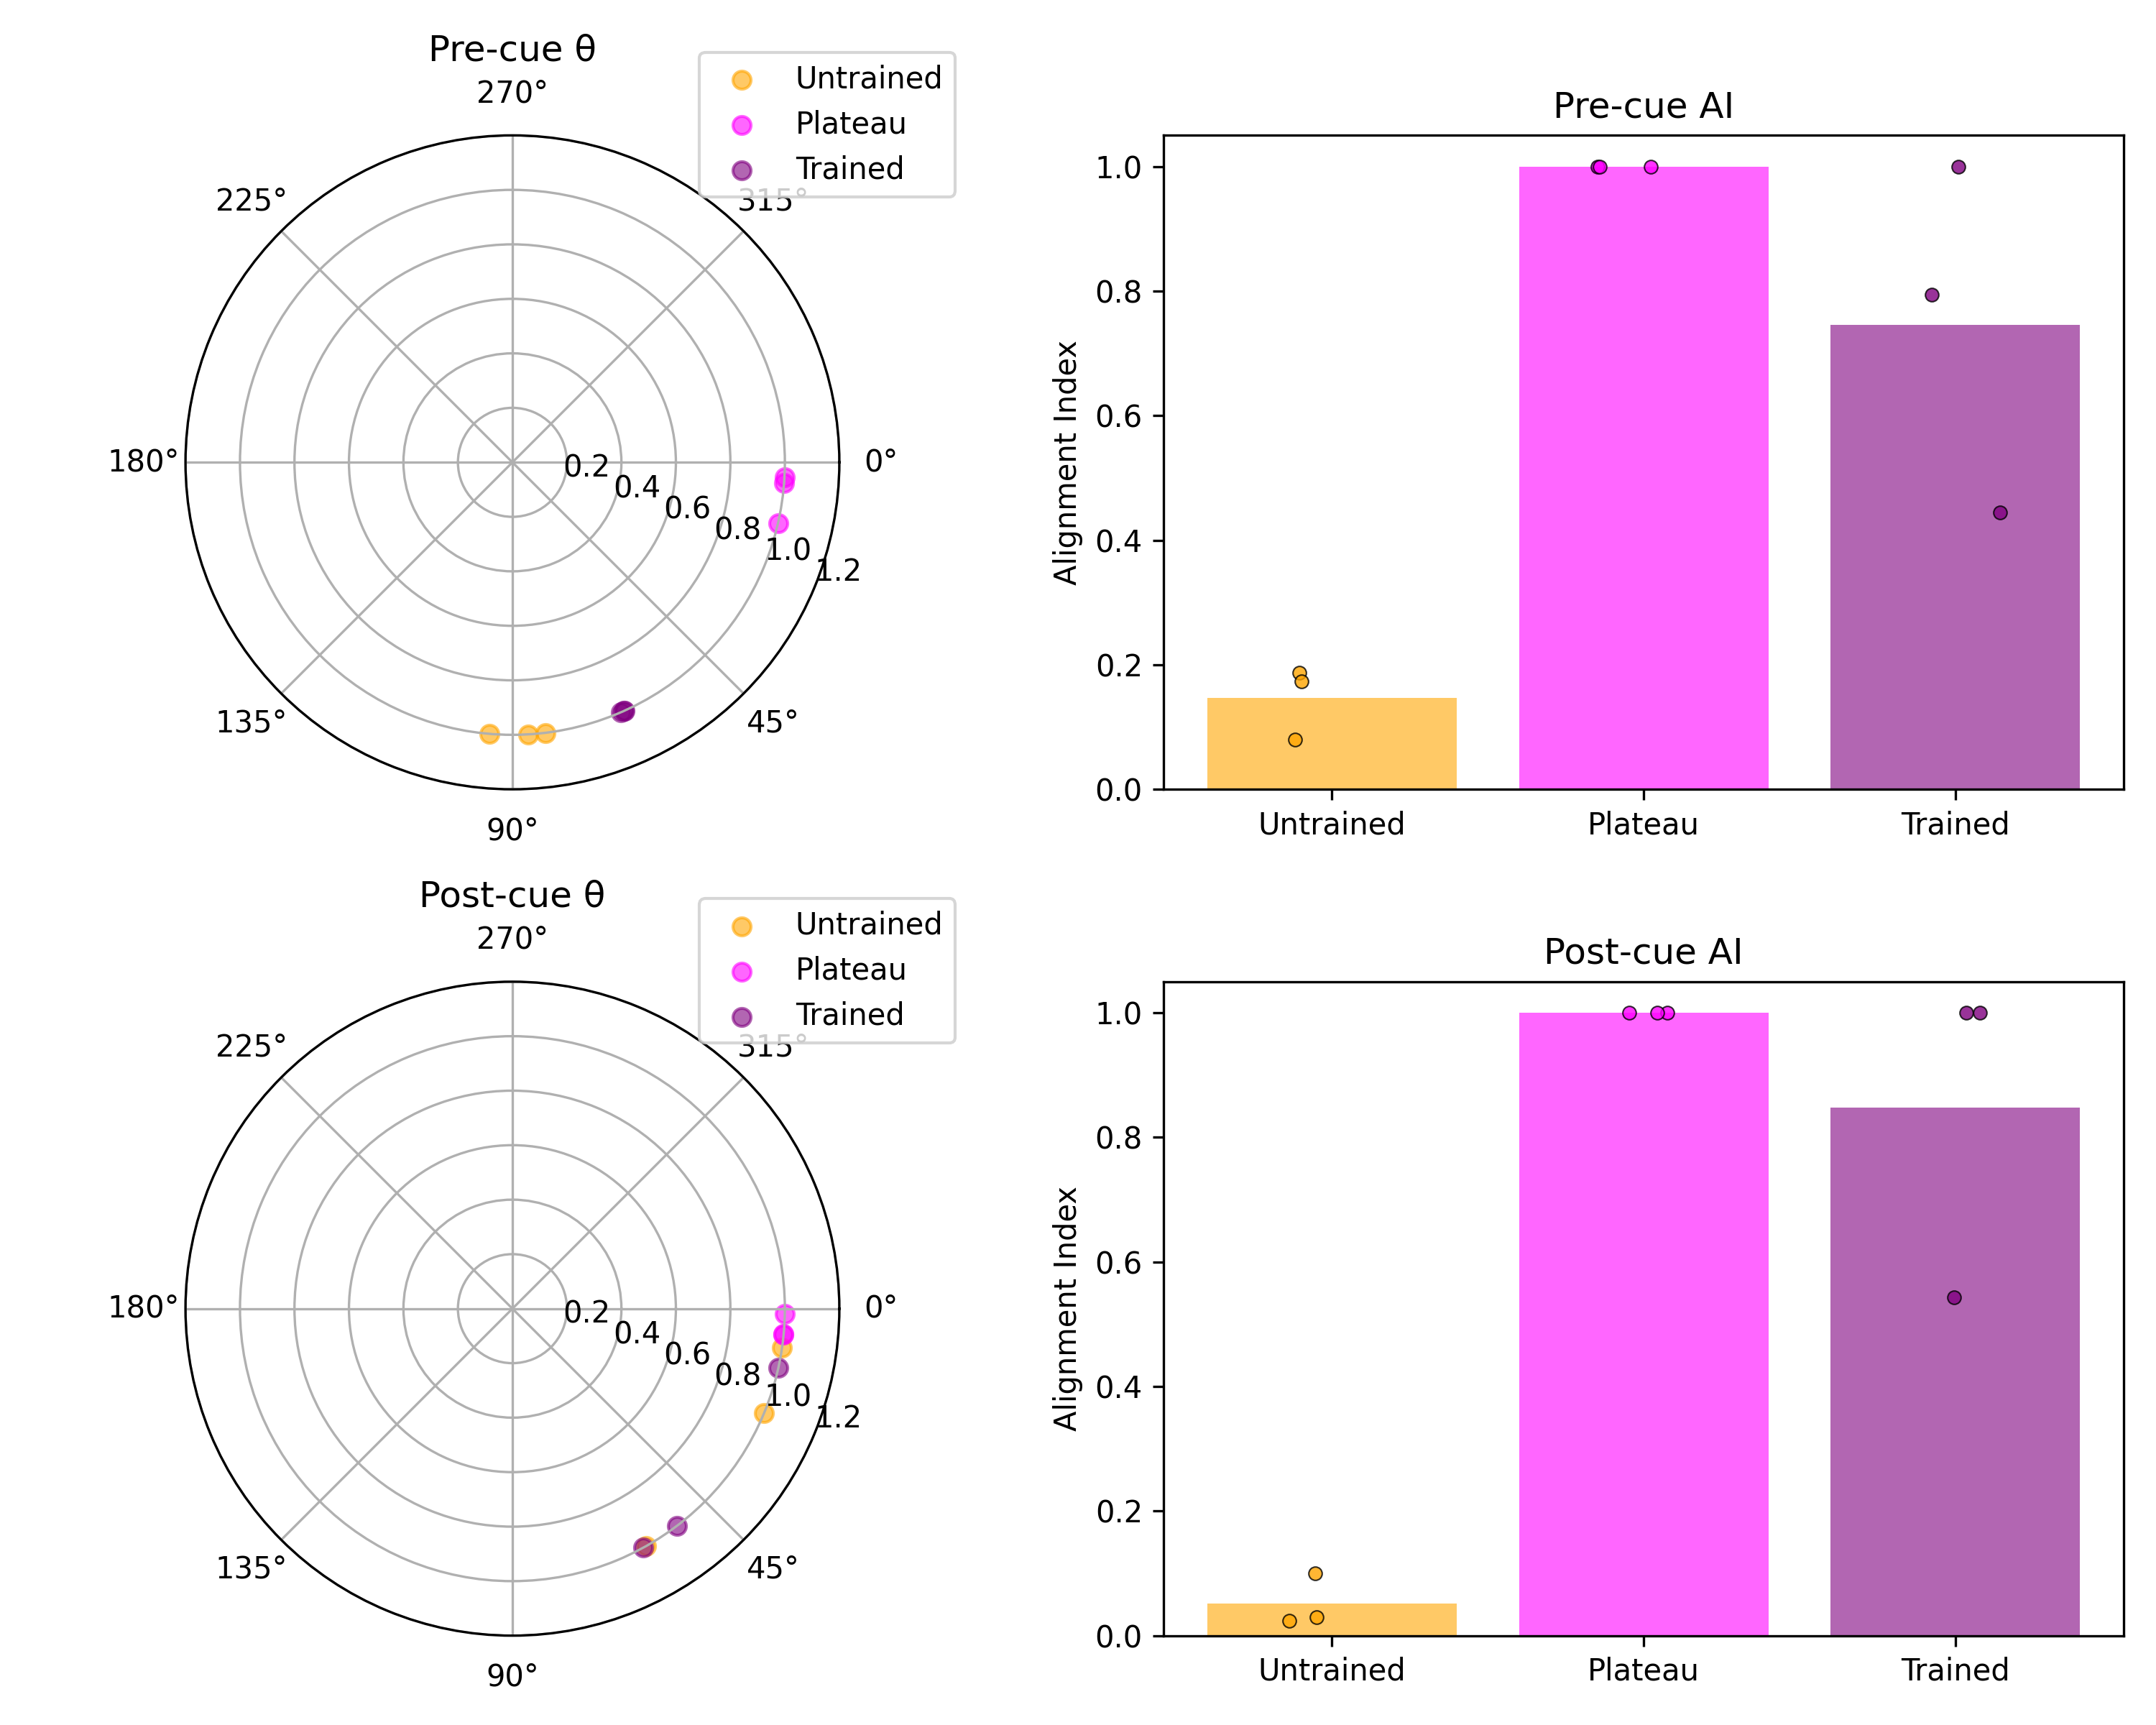
\includegraphics[width=0.48\textwidth]{fig4C_angles_ai.png}
    \caption{Left: Fig.~2B plane visualisation (pre/post). Right: Fig.~4C polar plane angles and AI bars with jittered points.}
\end{figure}

\begin{figure}[h]
    \centering
    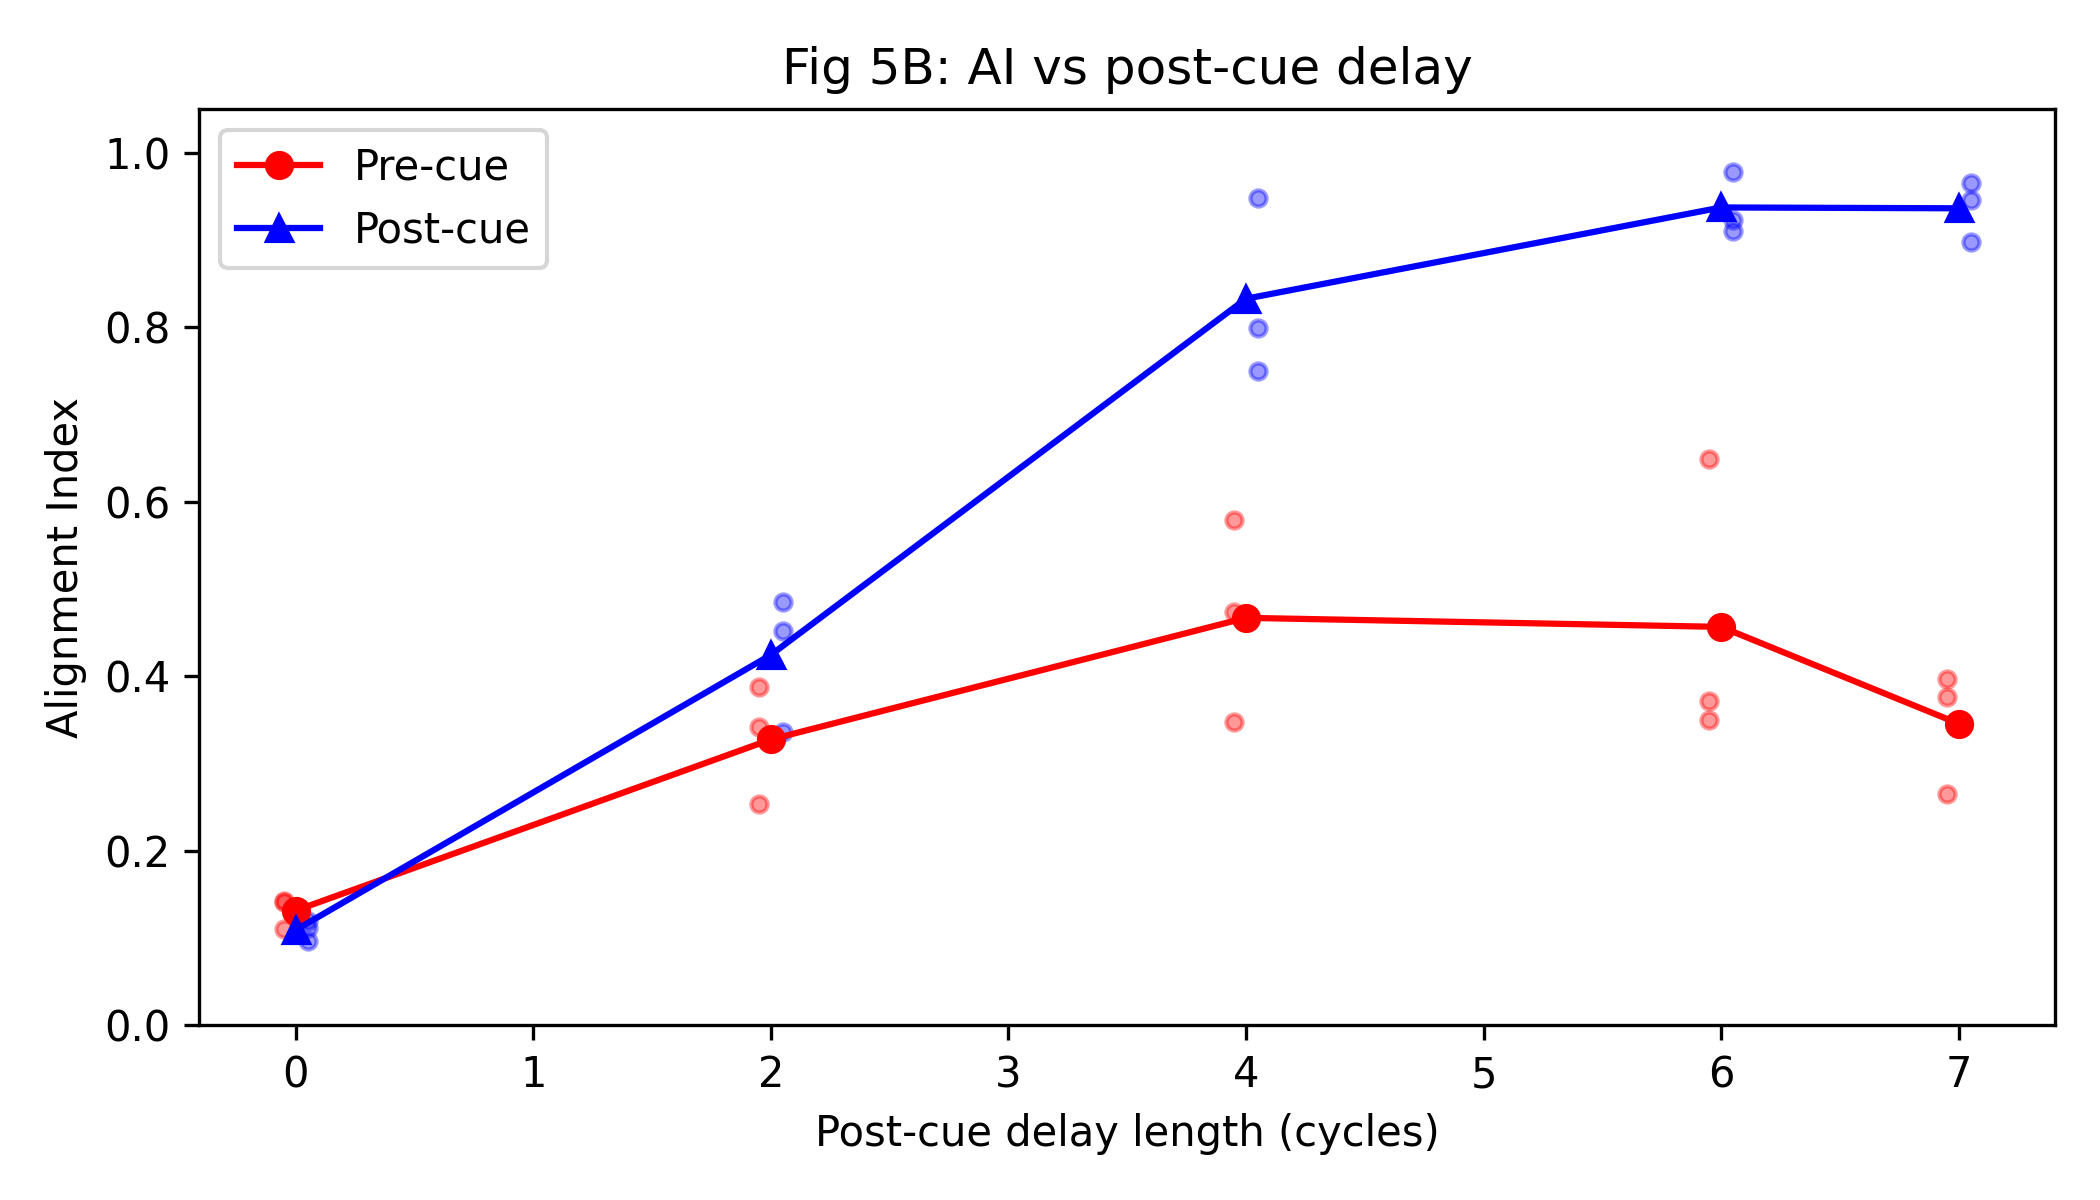
\includegraphics[width=0.7\textwidth]{fig5B_alignment_vs_delay.png}
    \caption{Fig.~5B replication: post-cue AI versus post-cue delay length (single replicate per condition).}
\end{figure}

\end{document}

